\section{Auswertung}
\label{sec:Auswertung}

\subsection{Einseitige Einspannung}
\subsubsection{Eckiger Stab}
Die Daten des eckigen Stabes, Länge $L$, Breite $b$ und Höhe $d$, ergeben sich zu:
\begin{align*}
  L &= \SI{60.04\pm 0.01}{\centi\metre}\\
  b &= \SI{1.036\pm 0.003}{\centi\metre}\\
  d &= \SI{1.016\pm0.002}{\centi\metre}
\end{align*} 
Das Gewicht, welches benutzt wurde, wiegt:
\begin{equation*}
  m = \SI{1.1003}{\kilo\gram}
\end{equation*}
\begin{table}
  \centering
  \caption{Die einzelnen Messungen des eckigen Stabes}
  \label{tab:5mess_eckig}
  \begin{tabular}{
    S[table-format=2.2] %länge
    S[table-format=1.2] %breite
    S[table-format=1.2]}
  \toprule
  {$ L \mathbin{/} \si{\centi\metre} $} &
  {$ b \mathbin{/} \si{\centi\metre} $} &
  {$ d \mathbin{/} \si{\centi\metre} $}\\
  \midrule
  60& 1.03 & 1.01\\
  60&1.06&1.02\\
  60.1&1.01&1.01\\
  60.1&1.05&1.01\\
  60&1.03&1.03\\
  \bottomrule
  \end{tabular}
\end{table}

\begin{table}
  \centering
  \caption{Messwerte zur einseitigen Einspannung eines eckigen Stabes}
  \label{tab:eckig}
  \begin{tabular}{S[table-format=3.0] 
                  S[table-format=1.2]
                  S[table-format=1.2] 
                  S[table-format=1.2]
                  S[table-format=3.2]}
    \toprule
    {$x \mathbin{/} \si{\milli\metre}$}&
    {$D_0 \mathbin{/} \si{\milli\metre}$}&
    {$D \mathbin{/} \si{\milli\metre}$}&
    {$\Delta D \mathbin{/} \si{\milli\metre}$}&
    {$Lx^2 - \frac{x^3}{3} \mathbin{/} \SI{e-3}{\metre\tothe{3}}$}\\
    \midrule
    25  &    0.73 &   0.75 &   0.02 & 0.37\\
    50   &   0.75 &   0.84 &   0.09 & 1.46 \\
    75   &   0.78 &   0.98 &   0.20 & 3.24\\
    100  &   0.83 &   1.15 &   0.32 & 5.67\\
    125  &   0.94 &   1.44 &   0.50 & 8.73\\
    150  &   0.98 &   1.67 &   0.69 & 12.38\\
    175  &   0.14 &   1.04 &   0.90 & 16.60\\
    200  &   0.22 &   1.32 &   1.10 & 21.35\\
    225  &   0.38 &   1.76 &   1.38 & 26.60\\
    250  &   0.54 &   2.21 &   1.67 & 32.32\\
    275  &   0.28 &   2.23 &   1.95 & 38.47\\
    300  &   0.37 &   2.66 &   2.29 & 45.04\\
    325  &   0.40 &   3.03 &   2.63 & 51.97\\
    350  &   0.41 &   3.37 &   2.96 & 59.26\\
    375  &   0.47 &   3.81 &   3.34 & 66.85\\
    400  &   0.55 &   4.21 &   3.66 & 74.73\\
    425  &   0.64 &   4.69 &   4.05 & 82.86\\
    450  &   0.73 &   5.14 &   4.41 & 91.21\\
    475  &   0.82 &   5.62 &   4.80 & 99.74\\
    500  &   0.82 &   5.97 &   5.15 & 108.43\\
    \bottomrule
  \end{tabular}
\end{table}
Für $y=(L\cdot x^2 - \frac{x^3}{3})$ werden die Messwerte in ein $y-\Delta D$ -Diagramm eingetragen.
Der lineare Zusammenhang wird mit einer Ausgleichsrechnung der Form $\Delta D(y)= a \cdot x + c $ mit ipython genauer untersucht.
Es ergeben sich: 
\begin{align*}
  a &= \SI{4.79(4)e-8}{\per\milli\metre\squared} & c&= \SI{0.07 \pm 0.02}{\milli\metre}
\end{align*}

\begin{figure}
  \centering
  \caption{Der eckige Stab unter einseitiger Einspannung.}
  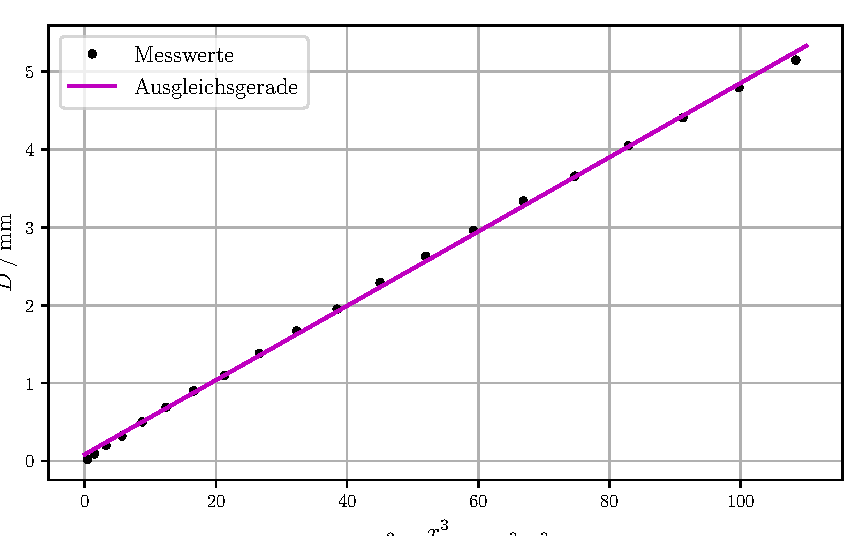
\includegraphics[width=\textwidth]{build/plotk.pdf}
  \label{fig:eckig}
\end{figure}
Nach Vergleich von \eqref{eqn:einseitig}
und der Ausgleichsrechnung folgt, dass sich das Elastizitätsmodul so berechnen lässt:
\begin{equation*}
  E = \frac{F}{2 \cdot I \cdot a} 
\end{equation*}
Für $F$ gilt $F = m \cdot g$ mit $g=\SI{9.81}{\metre\per\second\squared}$, das Flächenträgheitsmoment $I$ errechnet sich zu:
\begin{equation*}
  I = \frac{b\cdot d}{12} (b^2 + d^2) = \SI{0.923(70)e-9}{\metre\tothe{4}}
\end{equation*}
Somit ergibt sich für das Elastizitätsmodul des eckigen Stabes:
\begin{equation*}
  E = \SI{122.2(13)e9}{\newton\per\metre\squared}
\end{equation*}
Vermutlich handelt es sich bei dem eckigen Stab um einen Kupferstab. Der Literaturwert lautet nach \cite{chemie.de}
$E_{\text{Cu}} = \SI{120}{\kilo\newton\per\milli\metre\squared} = \SI{120e9}{\newton\per\metre\squared}$. 
Die Abweichung ergibt sich zu $\SI{1.83}{\percent}$.  


\subsubsection{Runder Stab}
Die Länge und der Radius des runden Stabes ergeben sich zu
\begin{align*}
  L &= \SI{60.03\pm 0.008}{\centi\metre} & r &= \SI{0.545\pm 0.0006}{\centi\metre}, 
\end{align*}
die Masse des Gewichtes zu 
\begin{equation*}
  m = \SI{599.6}{\gram}.
\end{equation*}
\begin{table}
  \centering
  \caption{Die einzelnen Messungen des runden Stabes.}
  \label{tab:5mess_rund}
  \begin{tabular}{
      S[table-format=2.2]
      S[table-format=1.2]}
  \toprule
  {$ L \mathbin{/} \si{\centi\metre} $} &
  {$ r \mathbin{/} \si{\centi\metre} $} \\
  \midrule
  60& 1.1\\
  60&1.09\\
  60&1.08\\
  60.1&1.09\\
  60.05&1.09\\
  \bottomrule
  \end{tabular}
\end{table}
\begin{table}
  \centering
  \caption{Die Messwerte der einseitigen Einspannung eines runden Stabes.}
  \label{tab:rund_einseitig}
  \begin{tabular}{S[table-format=3.0]
                  S[table-format=1.2]
                  S[table-format=1.2]
                  S[table-format=1.2]
                  S[table-format=3.2]}
    \toprule
    {$x \mathbin{/} \si{\milli\metre}$}&
    {$D_0 \mathbin{/} \si{\milli\metre}$}&
    {$D \mathbin{/} \si{\milli\metre}$}&
    {$\Delta D \mathbin{/} \si{\milli\metre}$}&
    {$Lx^2 - \frac{x^3}{3} \mathbin{/} \SI{e-3}{\metre\tothe{3}}$}\\
    \midrule
     25   & 0.55   & 0.58  &  0.03   & 0.37\\
     50     & 0.43   & 0.54  &  0.11 & 1.46\\
     75   & 0.33   & 0.56  &  0.23  & 3.24\\
    100     & 0.23   & 0.62  &  0.39 & 5.67\\
    125   & 0.13   & 0.71  &  0.58 & 8.73\\
    150     & 0.02   & 0.83  &  0.81 & 12.38\\
    175   & 0.98   & 2.05  &  1.07 & 16.60\\
    200     & 0.90   & 2.20  &  1.30 & 21.35\\
    225   & 0.75   & 2.44  &  1.69 & 26.60\\
    250     & 0.67   & 2.71  &  2.04 & 31.10\\
    275   & 0.62   & 3.01  &  2.39 & 38.47\\
    300     & 0.60   & 3.28  &  2.68 & 45.03\\
    325   & 0.55   & 3.62  &  3.07 & 51.96\\
    350     & 0.55   & 3.93  &  3.38 & 59.25\\
    375   & 0.36   & 4.34  &  3.98 & 66.84\\
    400     & 0.45   & 4.87  &  4.42 & 74.71\\
    425   & 0.46   & 5.15  &  4.69 & 82.84\\
    450     & 0.50   & 5.55  &  5.05 & 91.18\\
    475   & 0.50   & 6.12  &  5.62 & 99.72\\
    500     & 0.39   & 6.53  &  6.14 & 108.41\\
    \bottomrule
  \end{tabular}
\end{table}
Mit den Messwerten aus \ref{tab:rund_einseitig} wurde analog zum eckigen Stab der Auslenkungsunterschied $\Delta D$, im folgenden mit $D$ benannt, gegen den Ausdruck $L\cdot x^2 - \frac{x^3}{3}$, im folgenden mit $y$ benannt, in einem Diagramm aufgetragen.
Es wurde eine Ausgleichsrechnung für einen linearen Zusammenhang $D(y) = a\cdot y + c $ mit ipython durchgeführt.
Für die Funktionskonstanten ergeben sich:
\begin{align*}
  a &= \SI{5.59(6)e-8}{\per\milli\metre\squared}& c &= \SI{0.12\pm 0.03}{\milli\metre}
\end{align*}

\begin{figure}
  \centering
  \caption{Der runde Stab unter einseitiger Einspannung.}
  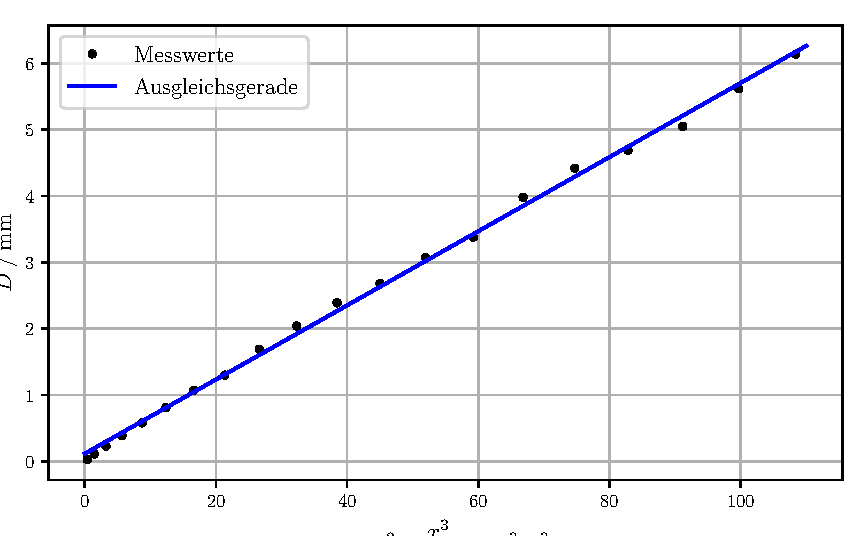
\includegraphics[width=\textwidth]{build/plotm1.pdf}
  \label{fig:plot1m}
\end{figure}
Das Elastizitätsmodul $E$ lässt sich nach \eqref{eqn:einseitig}
wie folgt berechnen:
\begin{equation*}
  E = \frac{F}{2 \cdot I \cdot a}
\end{equation*}
Für das Flächenträgheitsmoment des runden Stabes ergibt sich
\begin{equation}\label{eqn:Trägheitsmoment_rund}
  I = \frac{\pi \cdot r^4}{4} = \SI{6.93(3)e-10}{\metre\tothe{4}}
\end{equation} 
und $F$ ist gegeben als $F = m \cdot g$ mit $g = \SI{9.81}{\metre\per\second\squared}$.
Somit ist 
\begin{equation*}
  E = \SI{75.9(9)e9}{\newton\per\metre\squared}
\end{equation*}
Es wird davon ausgegangen, dass es sich bei dem runden Stab um Messing handelt.
Der Literaturwert des Elastizitätsmodul für Messing wird in \cite{chemie.de} als Bereich von $\num{78}$ bis $\SI{123}{\kilo\newton\per\milli\metre\squared}$ angegeben.
Der hier errechnete Wert liegt somit knapp unterhalb des Bereiches.

\subsection{Beidseitige Einspannung}
In dieser Methode wurde nur der runde Stab gemessen. Die Daten des Stabes lauten:
\begin{align*}
  L &= \SI{60.03\pm 0.008}{\centi\metre} & r &= \SI{0.545\pm 0.0006}{\centi\metre}
\end{align*}
Die einzelnen Messungen bezüglich der Länge und des Radius sind hier \ref{tab:5mess_rund} zu finden. 
Es wurde ein Gewicht der Masse 
\begin{equation*}
  m = \SI{1099.5}{\gram}
\end{equation*}
benutzt. Dieses lag bei etwa $x = \SI{275}{\milli\metre}$ auf.

\begin{table}
  \centering
  \caption{Der runde Stab bei beidseitiger Einspannung.}
  \begin{tabular}{
    S[table-format=3.0]
    S[table-format=1.2]
    S[table-format=1.2]
    S[table-format=1.2]
    S[table-format=3.2]}
  \toprule
  {$x \mathbin{/} \si{\milli\metre}$}&
  {$D_0 \mathbin{/} \si{\milli\metre}$}&
  {$D \mathbin{/} \si{\milli\metre}$}&
  {$ \Delta D \mathbin{/} \si{\milli\metre}$}&
  {$3L^2x - 4x^3 \mathbin{/} \SI{e-3}{\metre\tothe{3}}$}\\
  \midrule
  25   &   0.48  &  0.50  &  0.02 &  26.96\\
  50   &   0.45  &  0.50  &  0.05 &  53.55\\
  100  &   0.39  &  0.54  &  0.15 &  104.11\\
  150  &   0.24  &  0.55  &  0.31 &  148.66\\
  200  &   0.08  &  0.56  &  0.48 &  184.22\\
  220  &   0.97  &  1.58  &  0.61 &  195.25\\
  250  &   0.96  &  1.59  &  0.63 &  207.77\\
  \midrule
  {$x \mathbin{/} \si{\milli\metre}$}&
  {$D_0 \mathbin{/} \si{\milli\metre}$}&
  {$D \mathbin{/} \si{\milli\metre}$}&
  {$ \Delta D \mathbin{/} \si{\milli\metre}$}&
  {$4x^3 - 12Lx^2 + 9L^2x - L^3 \mathbin{/} \SI{e-3}{\metre\tothe{3}}$}\\
  \midrule
  300  &   0.53  &  1.36  &  0.83 &   216.32\\
  325  &   0.52  &  1.32  &  0.80 &   214.16\\
  350  &   0.39  &  1.27  &  0.88 &   207.87\\
  400  &   0.30  &  1.20  &  0.90 &   184.40\\
  450  &   0.29  &  1.08  &  0.79 &   148.91\\
  500  &   0.23  &  1.11  &  0.88 &   104.40\\
  520  &   0.30  &  0.68  &  0.38 &   84.74\\
  \bottomrule
  \end{tabular}
  \label{tab: rund_beid}
\end{table}
Die eigentliche Auslenkung $ \Delta D$ wird im folgenden $D$ genannt und in einem Diagramm gegen $y $ aufgetragen. 
Mit ipython wird eine Ausgleichsrechnung der Form $D(y) = a \cdot y + c$ gemacht. \\
Für $0 \leq x \leq \frac{L}{2}$ ist $y= 3L^2x - 4x^3$ und die Funktionskonstanten:
\begin{align*}
  a_1 &= \SI{3.5(4)e-3}{\per\metre\squared} & c_1 &= \SI{-0.14 \pm 0.06}{\milli\meter}
\end{align*}
Für $\frac{L}{2} \leq x \leq L$ ist $y = 4x^3 -12Lx^2 + 9L^2x -L^3$ und die Funktionskonstanten ergeben sich zu:
\begin{align*}
  a_2 &= \SI{2.0(12)e-3}{\per\metre\squared} & c_2 &= \SI{0.44 \pm 0.21}{\milli\meter}
\end{align*}
\begin{figure}
  \caption{Der runde Stab unter beidseitiger Einspannung für $0 \leq x \leq \frac{L}{2}$.}
  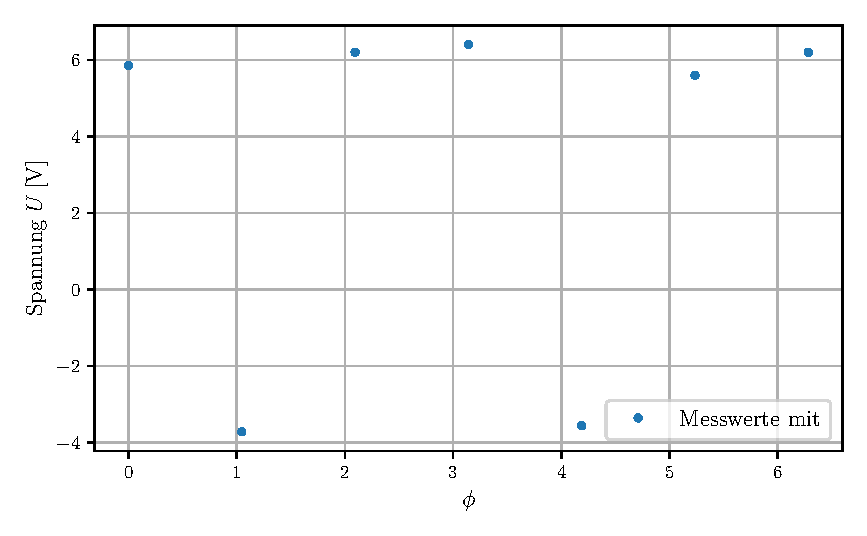
\includegraphics[width=\textwidth]{build/plot2.pdf}
\end{figure}
\begin{figure}
  \centering
  \caption{Der runde Stab unter beidseitiger Einspannung für $\frac{L}{2} \leq x \leq L$.}
  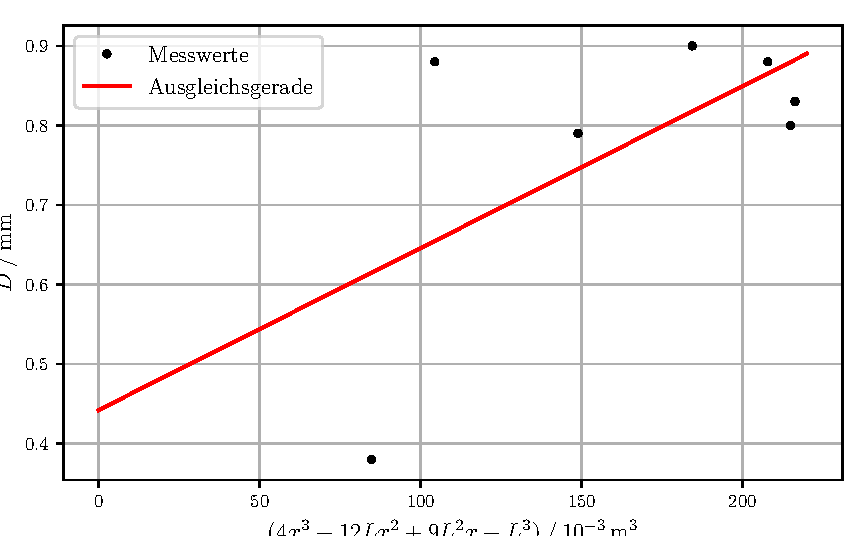
\includegraphics[width= \textwidth]{plot22.pdf}
  \label{fig:rund_beid2}
\end{figure}
Aus den Gleichungen \eqref{eqn:beidseitig1} und \eqref{eqn:beidseitig2} folgt, dass sich das Elastizitätsmodul wie folgt berechnen lässt:
\begin{equation*}
  E = \frac{F}{48 \cdot I \cdot a}
\end{equation*}
Dabei ist $F = m\cdot g$ und $I$ aus \eqref{eqn:Trägheitsmoment_rund} bekannt.
\begin{align*}
  E_1 &= \SI{93(10)e9}{\newton\per\metre\squared}\\
  E_2 &= \SI{160(90)e9}{\newton\per\metre\squared}
\end{align*}
Der Literaturwert vom Elastizitätsmodul von Messing kann laut \cite{chemie.de} $\num{78}$ bis $\SI{123}{\kilo\newton\per\milli\metre\squared}$ betragen. 
Der errechnete Wert $E_1$ liegt in diesem Bereich, der Wert von $E_2$ deutlich oberhalb des Bereiches. 